Like many online self-service platforms, the system architecture responsible for implementing the OZG relies on user profiles for managing identities. In case of the OZG, identity management is especially complicated due to the federated model of interoperable user profiles. Each member state has to provide its own user profile system which can be utilized through every administration portal. This solution is expensive to develop and maintain, as communication between multiple member states and institutions is required.







Goal of the integration solution is to introduce features of the IMP system into the OZG system architecture. All existing services should be accessible the same way as before but with additional options for using IMP. The focus of this initial integration is to avoid disruption of existing system operation through non-invasive integration, to enable a fast and simple introduction of IMP features and to provide future upgrade capabilities. The integration takes place on three layers:

\begin{figure}[h]
\caption{IMP Layer Diagram}
    \centering
    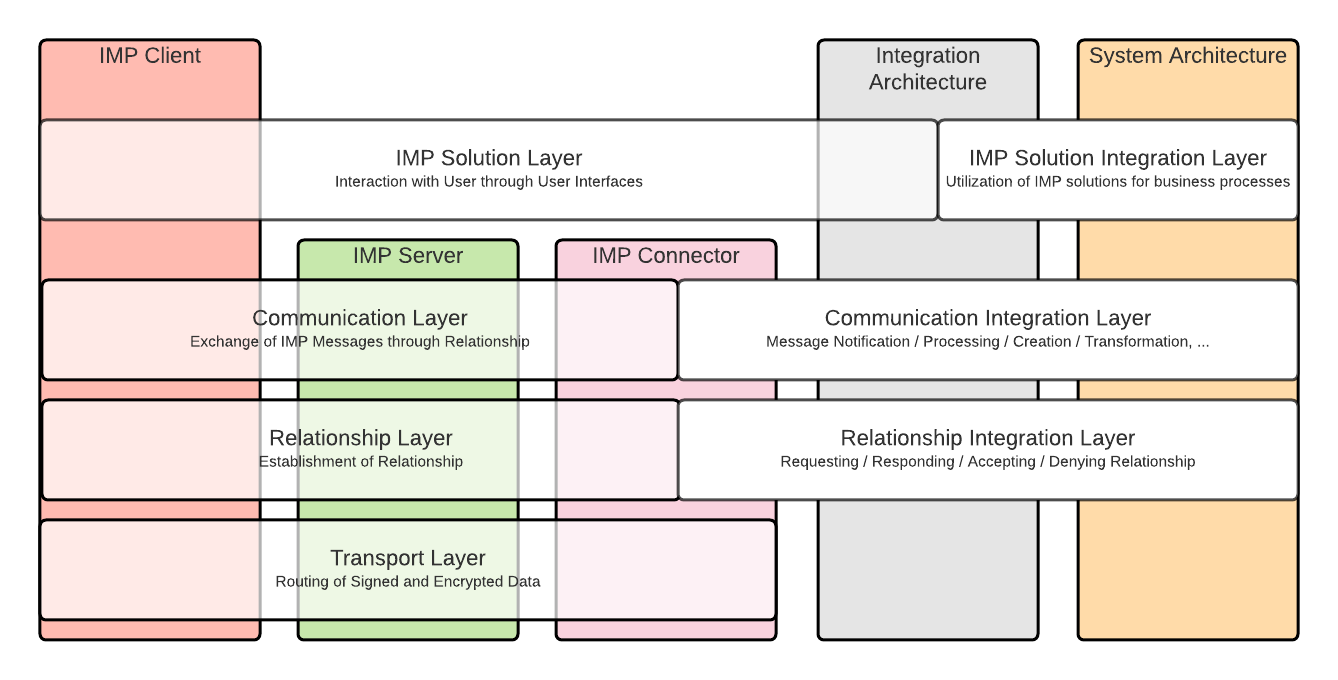
\includegraphics[scale=0.3]{Diagrams/Integration Architecture 1/IMP Layer Diagram Integration.png}
\end{figure}

\paragraph{IMP Solution Integration Layer} 
The purpose of the integration on the IMP solution layer is to take advantage of new interaction capabilities with the user through the IMP system. The integration evaluates possibilities of using relationships and IMP messages to improve OZG services, defines what the purpose of each message and relationship type is and how they should be handled by client and service provider. For example relationship templates can be defined and new message types can be created with corresponding new user interfaces in the IMP client.

\paragraph{Relationship Integration Layer} The purpose of the integration on the relationship layer is to enable the technological utilization of relationships as described by the integration on the solution integration layer. 

\paragraph{Communication Integration Layer} The purpose of the integration on the communication layer is to enable the technological utilization of messages as described by the integration on the solution integration layer.

\section{IMP Solution Integration}

\subfile{10-imp_solution_integration}

\section{Technological Integration}

This section evaluates possibilities of a technological integration architecture for realizing the integration solution described in the previous section.

\subfile{11-technological_integration}